\documentclass[journal]{IEEEtran}

\usepackage{amsmath,amssymb}
\usepackage{array}
\usepackage{booktabs}
\usepackage{cite}
\usepackage{multirow}
\usepackage{tabularx}
\usepackage{tikz}
\usepackage{url}
\usepackage{xcolor}
\usepackage{pgfplots}
\usepgfplotslibrary{groupplots}
\usetikzlibrary{arrows.meta,calc,positioning}
\pgfplotsset{compat=1.18}

\definecolor{navy}{HTML}{243B53}
\definecolor{slate}{HTML}{5C6773}
\definecolor{teal}{HTML}{4F7773}
\definecolor{rust}{HTML}{8F5147}
\definecolor{graytext}{HTML}{60656B}
\definecolor{lightgray}{HTML}{E2E5E8}
\newcolumntype{L}[1]{>{\raggedright\arraybackslash}p{#1}}
\newcolumntype{Y}{>{\raggedright\arraybackslash}X}

\newcommand{\pp}{\,\text{percentage points}}

\title{A Negative Result for Training-Free Temporal Visual Caching in OpenVLA-OFT}

\author{Ved Dwivedi, Cheng Yang, and Bo Yuan%
\thanks{Ved Dwivedi is with John P. Stevens High School, Edison, NJ, USA.}%
\thanks{Cheng Yang and Bo Yuan are with the Department of Electrical and Computer Engineering, Rutgers University--New Brunswick, Piscataway, NJ, USA.}}

\markboth{Author-Review Manuscript for IEEE Transactions on Robotics}{Dwivedi \MakeLowercase{\textit{et al.}}: Training-Free Temporal Visual Caching in OpenVLA-OFT}

\begin{document}
\maketitle

\begin{abstract}
Vision--language--action (VLA) policies repeatedly process similar visual observations during robot manipulation, making temporal reuse a potential approach for reducing inference cost. However, reused representations may omit task-relevant changes and alter subsequent closed-loop behavior. We present a systematic evaluation of three training-free temporal reuse strategies in OpenVLA-OFT on LIBERO: complete visual-prefix reuse, scene-camera reuse with wrist-camera refresh, and selective reuse of visual key--value states across transformer layers and image regions. Complete-prefix reuse was evaluated over 1,160 closed-loop episodes. Settings that skipped visual refresh on 34.69--83.68\% of policy queries achieved only 0--52\% task success. Conservative refresh rules achieved 69 successes in 70 episodes but skipped visual refresh on only 0.95\% of policy queries. Scene-camera reuse matched the observed success count of batched dense inference at 67/70 while reusing the scene representation on 25.24\% of queries, but it provided no end-to-end latency improvement. Mean query time was 1,190.97~ms, compared with 1,188.28~ms for dense inference. Fine-grained key--value reuse reduced median complete-query time by 22.60\% in a controlled systems test but achieved 0/120 closed-loop successes, compared with 68/120 for dense inference from the same initial conditions. These findings show that training-free reuse at the tested representation boundaries did not provide a reliable success--latency tradeoff. They motivate reuse mechanisms that preserve current task-relevant information and policies trained explicitly to tolerate stale representations.
\end{abstract}

\begin{IEEEkeywords}
Vision--language--action models, robot learning, inference efficiency, temporal caching, closed-loop control.
\end{IEEEkeywords}

\section{Introduction}
\IEEEPARstart{V}{ision--language--action} (VLA) models map visual observations, language instructions, and robot state to actions. Recent systems have improved generalization across manipulation tasks, but their large visual encoders and language-model backbones make inference expensive~\cite{brohan2023rt1,zitkovich2023rt2,kim2025openvla}. OpenVLA-OFT improves action-generation efficiency through continuous action prediction, parallel decoding, and action chunking~\cite{kim2025oft}. Even with these improvements, the model processes the visual input again at every policy query.

Consecutive observations in manipulation often share the same background and many of the same objects. This temporal redundancy motivates caching visual tokens or transformer key--value (K/V) states across queries. VLA-Cache, for example, reports that static visual tokens can be reused while task-relevant tokens are recomputed~\cite{xu2025vlacache}. Other work accelerates VLA inference through visual token selection, model pruning, or reuse within an iterative action head~\cite{yang2025efficientvla}. These results establish that substantial redundancy exists. They also raise a system-specific question: when visual features are reused in an autoregressive VLA with action chunking, does the resulting policy preserve closed-loop task performance?

The difficulty is not captured by image similarity alone. A small change in a cached representation can change an action chunk. That action changes the robot state and the next camera observation. Later cache decisions are then made on a trajectory generated by the modified policy rather than the dense policy. Offline comparisons on dense-policy trajectories cannot reproduce this feedback.

We study this issue with one released OpenVLA-OFT checkpoint and the LIBERO simulator~\cite{liu2023libero}. The experiments progress from coarse to fine reuse. We first cache the complete projected representation of both cameras and trigger refreshes using image, robot-state, action, and cache-age signals. We then keep the wrist-camera representation current and reuse only the scene-camera representation. Finally, we reuse selected K/V states by layer and image region while recording the physical query from which every reused state originated.

The experiments consistently expose a reliability--efficiency boundary. Aggressive complete-prefix reuse reduces task success. Conservative refresh rules preserve success only when reuse becomes rare. Camera-selective reuse preserves success at a useful logical reuse rate, but its latency advantage disappears against a batched dense implementation. Fine-grained K/V reuse yields measurable computational savings but fails closed-loop control in the final paired evaluation. Together, these experiments provide an empirical characterization of a failure mode that is easy to miss when caching is evaluated only through token counts, component timings, or offline action similarity.

\begin{figure*}[t]
\centering
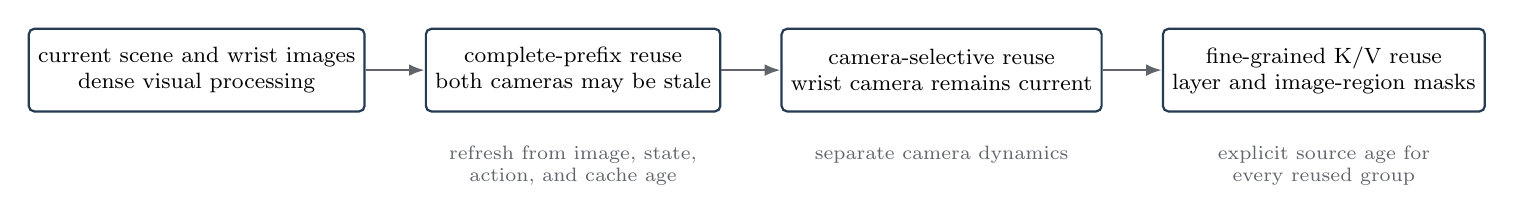
\begin{tikzpicture}[
  block/.style={draw=navy,rounded corners=2pt,minimum width=3.15cm,minimum height=1.05cm,align=center,font=\footnotesize,fill=white,line width=0.8pt},
  arrow/.style={-{Latex[length=2mm]},line width=0.9pt,draw=graytext},
  note/.style={font=\scriptsize,text=graytext,align=center}
]
\node[block] (dense) {current scene and wrist images\\dense visual processing};
\node[block,right=0.75cm of dense] (prefix) {complete-prefix reuse\\both cameras may be stale};
\node[block,right=0.75cm of prefix] (camera) {camera-selective reuse\\wrist camera remains current};
\node[block,right=0.75cm of camera] (kv) {fine-grained K/V reuse\\layer and image-region masks};
\draw[arrow] (dense) -- (prefix);
\draw[arrow] (prefix) -- (camera);
\draw[arrow] (camera) -- (kv);
\node[note,below=3mm of prefix] {refresh from image, state,\\action, and cache age};
\node[note,below=3mm of camera] {separate camera dynamics};
\node[note,below=3mm of kv] {explicit source age for\\every reused group};
\end{tikzpicture}
\caption{The three temporal reuse mechanisms evaluated in this study. Each mechanism retains more current information than the one before it.}
\label{fig:overview}
\end{figure*}

\section{Related Work}
\subsection{Vision--language--action policies}
RT-1 and RT-2 demonstrated large-scale language-conditioned visuomotor policies and transfer from vision--language pretraining~\cite{brohan2023rt1,zitkovich2023rt2}. OpenVLA provides an open 7B-parameter VLA built from fused DINOv2 and SigLIP visual features and a Llama-family language backbone~\cite{kim2025openvla}. OpenVLA-OFT replaces discrete action-token generation with a continuous action head and predicts action chunks in parallel~\cite{kim2025oft}. We use the released OpenVLA-OFT inference stack because it provides a public checkpoint, an official evaluator, and a strong dense baseline on LIBERO.

\subsection{Efficient VLA inference}
VLA inference can be accelerated by reducing model depth, processing fewer current-frame tokens, or reusing intermediate computation. EfficientVLA combines language-layer pruning, task-aware visual token selection, and feature caching within a diffusion action head~\cite{yang2025efficientvla}. VLA-Cache identifies visually stable tokens, excludes task-relevant regions using attention, and varies reuse across decoder layers~\cite{xu2025vlacache}. Recent work also studies learned token-selection policies that are optimized with the task objective~\cite{wei2026learnedcache}. These methods differ in architecture, cache location, and evaluation platform. Their published speedups are therefore not direct numerical baselines for our OpenVLA-OFT implementation.

Our study focuses on cross-query reuse in a closed-loop, action-chunked policy. The main distinction is between current-frame compression, which still derives every retained token from the current observation, and temporal reuse, which inserts representations computed from an earlier observation. The latter introduces representation age and can alter the state distribution encountered during control.

\subsection{Closed-loop distribution shift}
Sequential imitation learning distinguishes the state distribution generated by the reference policy from the distribution generated by a modified policy~\cite{ross2011dagger}. Let $d_{\pi_D}$ denote the state distribution induced by dense inference and $d_{\pi_C}$ the distribution induced by a cached policy. An offline comparison generally samples from $d_{\pi_D}$, whereas deployment evaluates states from $d_{\pi_C}$. Once cached inference changes an action,
\begin{equation}
    d_{\pi_C}(s) \neq d_{\pi_D}(s)
    \label{eq:shift}
\end{equation}
in general. This motivates direct closed-loop evaluation rather than treating offline action similarity as the final reliability measure.

\section{Problem Setting}
\subsection{Dense policy}
Let $q$ index policy queries. At query $q$, OpenVLA-OFT receives a language instruction $x$, a scene image $o_q^s$, a wrist image $o_q^w$, and proprioceptive state $p_q$. The visual encoder and projector produce visual tokens
\begin{equation}
    V_q = \mathcal{V}_{\theta}(o_q^s,o_q^w).
    \label{eq:visual}
\end{equation}
The transformer and continuous action head produce an eight-step, seven-dimensional action chunk
\begin{equation}
    A_q^D = h_{\theta}\!\left(\mathcal{T}_{\theta}(x,V_q,p_q)\right)
    \in \mathbb{R}^{8\times 7}.
    \label{eq:dense}
\end{equation}
The evaluator normally executes all eight actions before requesting another chunk. A changed prediction can therefore affect several environment transitions before the next cache decision.

\subsection{Temporal K/V reuse}
At transformer layer $\ell$ and visual group $g$, let $K_{q,\ell,g}$ and $U_{q,\ell,g}$ denote the K/V states computed from the current query. A binary mask $M_{q,\ell,g}=1$ selects the current states. If $M_{q,\ell,g}=0$, the cache uses states from a physical source query $\sigma(q,\ell,g)<q$:
\begin{align}
\widetilde K_{q,\ell,g} &= M_{q,\ell,g}K_{q,\ell,g}
 +(1-M_{q,\ell,g})K_{\sigma(q,\ell,g),\ell,g}, \\
\widetilde U_{q,\ell,g} &= M_{q,\ell,g}U_{q,\ell,g}
 +(1-M_{q,\ell,g})U_{\sigma(q,\ell,g),\ell,g}.
\label{eq:mix}
\end{align}
The source age is $a_{q,\ell,g}=q-\sigma(q,\ell,g)$. Recursive reuse can create one transformer state whose visual groups originate from different physical times.

\subsection{Evaluation measures}
For a fixed set of $N$ episodes, terminal task success is
\begin{equation}
    \widehat S(m)=\frac{1}{N}\sum_{i=1}^{N}
    \mathbb{1}\{\text{episode }i\text{ succeeds under method }m\}.
    \label{eq:success}
\end{equation}
We report exact two-sided 95\% binomial intervals for the central success results~\cite{clopper1934intervals}. These intervals do not model clustering by task or initial state.

For timing experiments, end-to-end improvement relative to dense inference is
\begin{equation}
    G_T(m)=1-\frac{T_m}{T_D},
    \label{eq:speed}
\end{equation}
where $T_m$ includes controller logic, cache management, synchronization, and data movement. We separately report the fraction of policy queries that reuse visual computation. Logical reuse and component-level CUDA time are mechanism measurements, not substitutes for end-to-end latency.

\section{Temporal Reuse Methods}
\subsection{Complete visual-prefix reuse}
The first method stores the projected scene and wrist visual tokens from the most recent refresh query $\tau_q$. It measures image change $d_q^{\mathrm{img}}$, normalized proprioceptive change $d_q^{\mathrm{state}}$, recent action change $d_q^{\mathrm{act}}$, and cache age $q-\tau_q$. The visual representation is refreshed when
\begin{equation}
 \begin{split}
 r_q=\mathbb{1}\!\left[
 d_q^{\mathrm{img}}>\gamma_I \vee
 d_q^{\mathrm{state}}>\gamma_S \right.\\
 \left. \vee\ d_q^{\mathrm{act}}>\gamma_A \vee
 q-\tau_q\ge H
 \right].
 \end{split}
 \label{eq:refresh}
\end{equation}
If $r_q=0$, the policy receives $V_{\tau_q}$ in place of $V_q$. We first use the average image change across both cameras. We then evaluate more conservative variants that threshold each camera separately, group state and action coordinates by physical meaning, prevent consecutive reuse, and force refreshes near gripper or motion-direction transitions.

\subsection{Camera-selective reuse}
Diagnostics from the complete-prefix experiments show that the wrist image often changes while the scene image remains stable. We therefore keep the wrist representation current and permit reuse only for the scene representation:
\begin{equation}
    \widetilde V_q = \left[V_{\tau_q}^{s};V_q^{w}\right].
    \label{eq:camera}
\end{equation}
On refresh queries, both cameras are processed as one batch. This batched dense path is the timing baseline because it avoids duplicated framework overhead without introducing stale information. The cache controller permits at most one reuse query before the next mandatory refresh.

\subsection{Fine-grained K/V reuse}
The final cache partitions each camera into a $4\times4$ grid and applies observation-dependent reuse masks at transformer layers 2, 6, 9, and 11. The maximum number of reusable scene-camera tokens increases from 48 to 192 of 256 tokens across these layers. The corresponding wrist-camera limits increase from 32 to 128 tokens. At least one region per camera remains current, scene states are at most four queries old, wrist states are at most two queries old, and the cache periodically resets to dense computation. The implementation records $\sigma(q,\ell,g)$ for every reused group so that the physical age in~\eqref{eq:mix} remains explicit.

We also explored whether an offline model could predict when fine-grained reuse would increase action error. Those exploratory targets were later found to depend on a custom action-extraction path that did not match the released evaluator. We therefore exclude the associated action-quality and risk-prediction results from the scientific analysis. Before the final fine-grained experiment, the custom dense path was corrected and independently verified to reproduce the released evaluator's hidden states and actions exactly.

\section{Experimental Protocol}
\subsection{Model, benchmark, and hardware}
All experiments use the released \texttt{openvla-7b-oft-libero-four-suite} checkpoint, two RGB cameras, current proprioception, and the official LIBERO terminal success function. The model runs on one NVIDIA TITAN RTX. The full-refresh experiments use LIBERO-Spatial. The paired camera-selective experiment uses LIBERO-Object. The final fine-grained cache experiment uses 30 initial conditions from each of the Spatial, Object, Goal, and LIBERO-10 suites.

The method families were developed sequentially and use different evaluation populations. We report their sample sizes separately and do not pool them into a single estimator. Paired comparisons use the same initial condition for dense and cached inference.

\begin{table*}[t]
\caption{Evaluation populations and primary measurements.}
\label{tab:protocol}
\centering
\footnotesize
\begin{tabularx}{\textwidth}{@{}L{3.4cm}L{3.0cm}L{3.2cm}YL{3.1cm}@{}}
\toprule
Reuse mechanism & Benchmark population & Closed-loop sample & Primary reliability measure & Efficiency measure \\
\midrule
Complete visual prefix & LIBERO-Spatial development states & 1,160 primary episodes & Terminal task success across threshold settings & Fraction of queries that skip visual refresh \\
Camera-selective visual prefix & LIBERO-Object paired states & 70 dense + 70 cached episodes & Paired terminal success & Complete wall time and visual CUDA time \\
Fine-grained K/V states & 30 paired states from each of four LIBERO suites & 120 dense + 120 cached episodes & Paired terminal success by suite & Median complete-query time reduction in the systems test \\
\bottomrule
\end{tabularx}
\end{table*}

\subsection{Timing baseline}
A separate 50-episode pilot measures 662 steady policy queries. Full refresh succeeds in 49/50 episodes. The visual encoder and projector require 201.19~ms per query, equal to 15.874\% of measured query CUDA time. Even a zero-overhead method that removed all visual work would therefore have a maximum speedup of approximately $1.189\times$ in this implementation. The pilot is not included in the 1,160 complete-prefix evaluation episodes.

\subsection{Implementation validation}
The final K/V experiment includes an independent comparison with the released OpenVLA-OFT evaluator. The test compares the hidden-state slice used by the continuous action head, normalized actions, and unnormalized actions. All three agree with maximum absolute error zero. Incomplete executions and measurements generated before this check are excluded from the reported final cache result.

\section{Results}
\subsection{Complete-prefix reuse}
Dense inference succeeds in all 100 baseline episodes used for the initial complete-prefix comparison. Across nine reuse settings, visual refresh is skipped on 34.69--83.68\% of policy queries, while terminal success ranges from 52/100 to 0/100. The best of these settings is 48 percentage points below dense inference.

Conservative refresh rules improve reliability but sharply reduce reuse. A configuration with no reuse succeeds in 30/30 episodes. Configurations with 6.72\% and 10.57\% reuse succeed in 29/30 and 27/30 episodes. The most conservative final configuration succeeds in 69/70 episodes but reuses the visual prefix on only 9 of 944 policy queries, or 0.9534\%.

\begin{table*}[t]
\caption{Representative complete-prefix results. Intervals are exact two-sided 95\% binomial intervals.}
\label{tab:prefix}
\centering
\footnotesize
\begin{tabular}{@{}lrrr@{}}
\toprule
Configuration & Success & 95\% interval & Reuse \\
\midrule
Dense reference & 100/100 & 96.38--100\% & 0\% \\
Best permissive setting & 52/100 & 41.78--62.10\% & 34.69\% \\
Highest-reuse setting & 0/100 & 0--3.62\% & 83.68\% \\
Conservative, no reuse & 30/30 & 88.43--100\% & 0\% \\
Conservative, moderate & 29/30 & 82.78--99.92\% & 6.72\% \\
Conservative, higher & 27/30 & 73.47--97.89\% & 10.57\% \\
Final conservative setting & 69/70 & 92.30--99.96\% & 0.95\% \\
\bottomrule
\end{tabular}
\end{table*}

The first reused query changes the predicted action in all 87 comparable episodes for which this diagnostic is available. Offline replay on dense-policy trajectories underestimates online reuse for every permissive setting. Camera averaging also obscures asymmetric change: 374 of 783 reuse decisions contain a threshold exceedance in at least one camera, and 372 of these cases are caused only by the wrist camera. These observations motivate the camera-selective experiment.

\begin{figure*}[t]
\centering
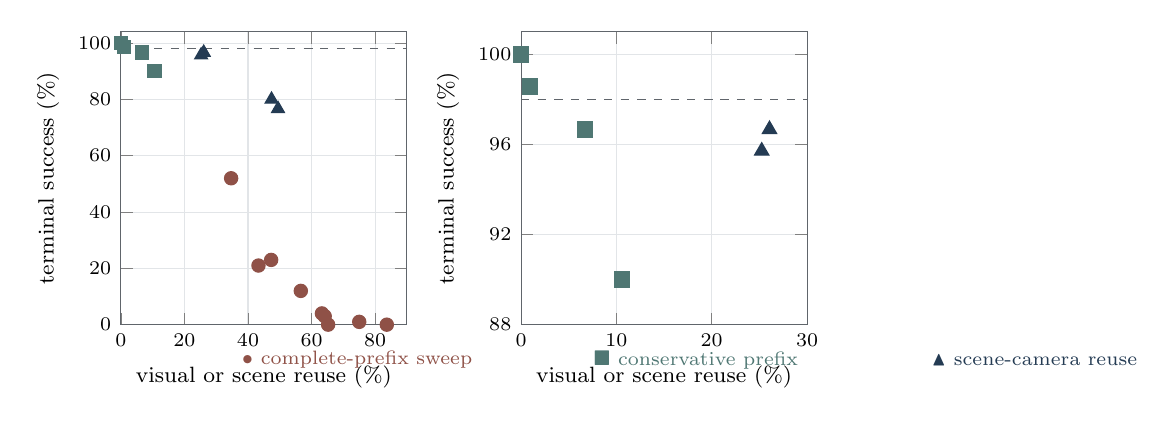
\begin{tikzpicture}
\begin{groupplot}[
 group style={group size=2 by 1,horizontal sep=1.45cm},
 width=0.43\textwidth,height=5.3cm,
 xmin=0,xmax=90,ymin=0,ymax=104,
 xlabel={visual or scene reuse (\%)},ylabel={terminal success (\%)},
 tick label style={font=\scriptsize},label style={font=\footnotesize},
 grid=major,grid style={draw=lightgray},axis line style={draw=graytext},
]
\nextgroupplot
\addplot[only marks,mark=*,mark size=2.4pt,rust] coordinates
 {(34.69,52)(43.29,21)(47.28,23)(56.62,12)(63.26,4)(65.21,0)(64.14,3)(75,1)(83.68,0)};
\addplot[only marks,mark=square*,mark size=2.4pt,teal] coordinates
 {(0,100)(6.72,96.67)(10.57,90)(0.9534,98.57)};
\addplot[only marks,mark=triangle*,mark size=2.7pt,navy] coordinates
 {(26.06,96.67)(47.40,80)(49.44,76.67)(25.2434,95.714)};
\addplot[graytext,dashed,domain=0:90] {98};
\nextgroupplot[xmin=0,xmax=30,ymin=88,ymax=101,ytick={88,92,96,100}]
\addplot[only marks,mark=square*,mark size=2.8pt,teal] coordinates
 {(0,100)(6.72,96.67)(10.57,90)(0.9534,98.57)};
\addplot[only marks,mark=triangle*,mark size=3pt,navy] coordinates
 {(26.06,96.67)(25.2434,95.714)};
\addplot[graytext,dashed,domain=0:30] {98};
\end{groupplot}
\node[font=\scriptsize,text=rust] at (3.0,-0.45) {$\bullet$ complete-prefix sweep};
\node[font=\scriptsize,text=teal] at (7.3,-0.45) {$\blacksquare$ conservative prefix};
\node[font=\scriptsize,text=navy] at (11.6,-0.45) {$\blacktriangle$ scene-camera reuse};
\end{tikzpicture}
\caption{Observed success--reuse operating points. The right panel enlarges the high-success region. Points summarize separate experimental populations and are therefore descriptive rather than randomized head-to-head estimates.}
\label{fig:frontier}
\end{figure*}

\subsection{Camera-selective reuse}
The initial camera-selective screen evaluates three 30-episode settings. They reuse the scene representation on 26.06\%, 47.40\%, and 49.44\% of queries and obtain 29/30, 24/30, and 23/30 successes, respectively. The most conservative setting therefore advances to a paired 70-episode comparison.

In the paired experiment, camera-selective reuse and batched dense inference each succeed in 67/70 episodes. The reuse policy retains an earlier scene representation on 25.24\% of queries. Relative to a sequential dense implementation, its mean wall time is 3.96\% lower. The relevant baseline is the batched dense implementation, however, because both camera images can be processed together without using stale information. Against this baseline, camera-selective reuse reduces visual CUDA time by 8.46\% but increases mean complete-query wall time from 1188.28 to 1190.97~ms. The 2.69~ms difference corresponds to a 0.23\% slowdown.

\begin{figure}[t]
\centering
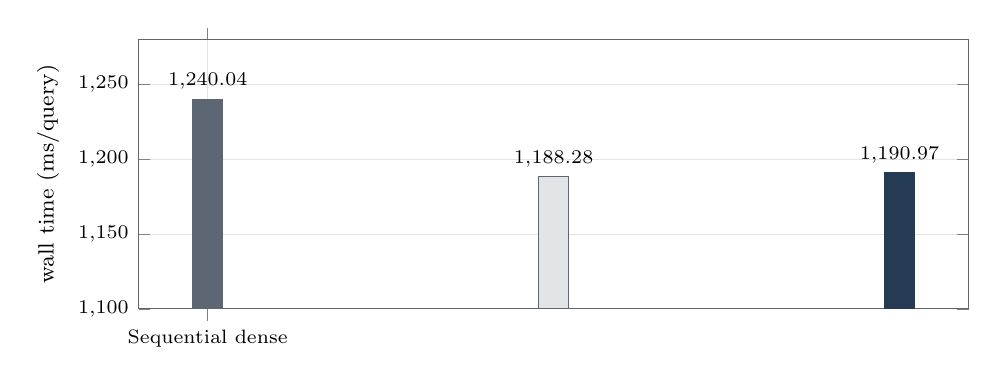
\begin{tikzpicture}
\begin{axis}[
 width=\columnwidth,height=5.0cm,
 ybar=0pt,bar width=11pt,
 ymin=1100,ymax=1280,
 ylabel={wall time (ms/query)},
 symbolic x coords={Sequential dense,Batched dense,Scene reuse},xtick=data,
 xticklabel style={font=\scriptsize,align=center},tick label style={font=\scriptsize},
 label style={font=\footnotesize},
 nodes near coords,nodes near coords style={font=\scriptsize},
 grid=major,grid style={draw=lightgray},axis line style={draw=graytext},
]
\addplot[fill=slate,draw=slate,bar shift=0pt] coordinates {(Sequential dense,1240.04)};
\addplot[fill=lightgray,draw=slate,bar shift=0pt] coordinates {(Batched dense,1188.28)};
\addplot[fill=navy,draw=navy,bar shift=0pt] coordinates {(Scene reuse,1190.97)};
\end{axis}
\end{tikzpicture}
\caption{Mean complete-query wall time in the paired camera-selective experiment. Reusing the scene representation does not improve latency relative to batched dense inference.}
\label{fig:camera_time}
\end{figure}

\subsection{Fine-grained K/V reuse}
The validated fine-grained cache reduces median complete-query time by 22.5969\% in a 97-call systems test. The paired closed-loop evaluation then runs dense and cached inference from the same 120 initial conditions, producing 240 episodes and 8,525 model queries. Dense inference succeeds in 68/120 episodes. Cached inference succeeds in 0/120 episodes, including 0/30 in each LIBERO suite. The overall dense--cache difference is 56.67 percentage points.

\begin{figure}[t]
\centering
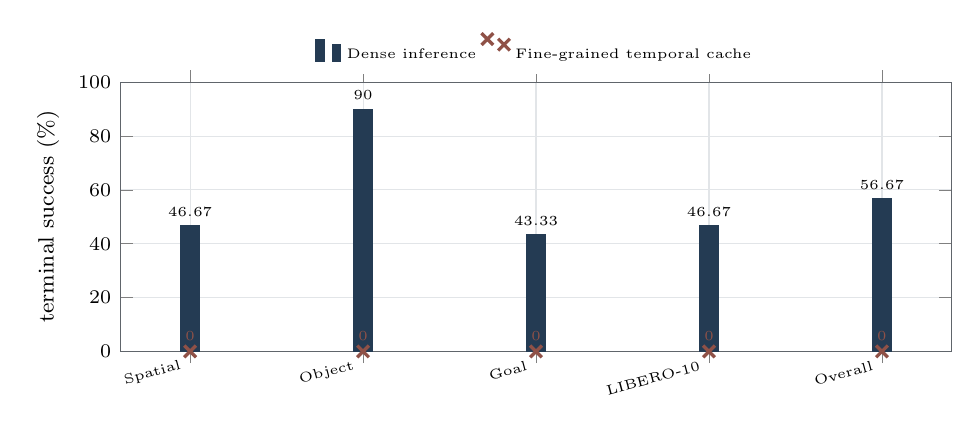
\begin{tikzpicture}
\begin{axis}[
 width=\columnwidth,height=5.0cm,
 ybar=1pt,bar width=7pt,
 ymin=0,ymax=100,ylabel={terminal success (\%)},
 symbolic x coords={Spatial,Object,Goal,LIBERO-10,Overall},xtick=data,
 xticklabel style={font=\tiny,rotate=15,anchor=east},tick label style={font=\scriptsize},
 label style={font=\footnotesize},
 legend style={font=\tiny,draw=none,at={(0.5,1.03)},anchor=south,legend columns=2},
 nodes near coords,nodes near coords style={font=\tiny},
 grid=major,grid style={draw=lightgray},axis line style={draw=graytext},
]
\addplot[fill=navy,draw=navy] coordinates
 {(Spatial,46.67)(Object,90)(Goal,43.33)(LIBERO-10,46.67)(Overall,56.67)};
\addplot[only marks,mark=x,mark size=3pt,rust,very thick] coordinates
 {(Spatial,0)(Object,0)(Goal,0)(LIBERO-10,0)(Overall,0)};
\legend{Dense inference,Fine-grained temporal cache}
\end{axis}
\end{tikzpicture}
\caption{Paired closed-loop success for dense inference and the validated fine-grained temporal cache. Each suite contains 30 episodes per condition.}
\label{fig:kv_success}
\end{figure}

\begin{table*}[t]
\caption{Paired closed-loop results for fine-grained K/V reuse. Intervals are exact two-sided 95\% binomial intervals.}
\label{tab:kv}
\centering
\scriptsize
\begin{tabular}{@{}lrrr@{}}
\toprule
Suite & Dense (95\% interval) & Cache (95\% interval) & Difference \\
\midrule
Spatial & 14/30 (28.34--65.67\%) & 0/30 (0--11.57\%) & $-46.67\pp$ \\
Object & 27/30 (73.47--97.89\%) & 0/30 (0--11.57\%) & $-90.00\pp$ \\
Goal & 13/30 (25.46--62.57\%) & 0/30 (0--11.57\%) & $-43.33\pp$ \\
LIBERO-10 & 14/30 (28.34--65.67\%) & 0/30 (0--11.57\%) & $-46.67\pp$ \\
Overall & 68/120 (47.31--65.68\%) & 0/120 (0--3.03\%) & $-56.67\pp$ \\
\bottomrule
\end{tabular}
\end{table*}

\section{Discussion}
\subsection{Visual similarity did not imply policy equivalence}
The complete-prefix results show that visually similar observations can still require different actions. All 87 examined episodes change their predicted action at the first reused query. The wrist-camera diagnostic gives a concrete explanation for part of this sensitivity. The wrist view changes with end-effector motion and object contact even when the global scene remains stable. Averaging the two camera-change signals hides this local change.

Keeping the wrist representation current substantially improves reliability. The paired camera-selective policy matches dense success while reusing the scene representation on one quarter of policy queries. This result shows that temporal reuse is not uniformly harmful. It also shows why success and speed must be measured together. The extra cache-control and execution paths cost more than the visual work they remove when compared with a batched dense baseline.

\subsection{Recursive K/V reuse changes the control state}
The fine-grained cache does not simply store independent image descriptors. At every transformer layer, the visual states interact with the instruction, proprioception, and action-query states. Reusing groups with different source ages therefore constructs an internal state that did not occur in dense inference. If that state changes an action chunk, the robot reaches a different observation. Recursive reuse then carries information from this altered trajectory into later queries.

\begin{figure*}[t]
\centering
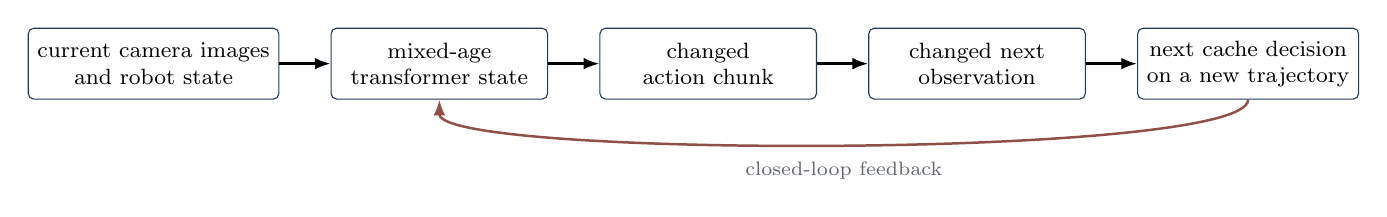
\begin{tikzpicture}[
 box/.style={draw=navy,rounded corners=2pt,minimum height=0.9cm,minimum width=2.75cm,align=center,font=\footnotesize,fill=white},
 arr/.style={-{Latex[length=2mm]},line width=0.9pt},
 note/.style={font=\scriptsize,text=graytext,align=center}
]
\node[box] (obs) {current camera images\\and robot state};
\node[box,right=0.65cm of obs] (mix) {mixed-age\\transformer state};
\node[box,right=0.65cm of mix] (act) {changed\\action chunk};
\node[box,right=0.65cm of act] (next) {changed next\\observation};
\node[box,right=0.65cm of next] (cache) {next cache decision\\on a new trajectory};
\draw[arr] (obs) -- (mix);
\draw[arr] (mix) -- (act);
\draw[arr] (act) -- (next);
\draw[arr] (next) -- (cache);
\draw[arr,rust] (cache.south) .. controls ($(cache.south)+(0,-0.75cm)$)
 and ($(mix.south)+(0,-0.75cm)$) .. node[note,below,yshift=-1mm]{closed-loop feedback} (mix.south);
\end{tikzpicture}
\caption{Temporal reuse can alter the trajectory on which later reuse decisions are made. Offline evaluation on dense-policy trajectories omits this feedback.}
\label{fig:feedback}
\end{figure*}

The final result is therefore stronger than an offline action-distance observation. The cache reduces measured query time yet fails every closed-loop episode. This does not prove that all K/V caching strategies will fail. It shows that the tested observation-dependent, mixed-age cache is not a usable operating point for this checkpoint and evaluator.

\subsection{The dense baseline determines whether a speedup is real}
The camera-selective experiment initially appears faster than sequential full refresh. Batching the two current camera images removes much of that apparent improvement without introducing staleness. A temporal cache should therefore be compared with a dense path that already uses batching, compiler optimization, quantization, and other compatible current-frame improvements. Otherwise, the reported speedup can reflect an avoidable implementation overhead rather than the caching method.

\subsection{Implications for future methods}
The results favor two directions. The first is current-frame compression, including task-aware token selection, token merging, quantization, and adaptive spatial resolution. These methods reduce computation while keeping the retained information tied to the present observation.

The second direction is cache-aware learning. If temporal reuse is required, the model can be trained with the same stale and recursively updated states that it will encounter at deployment. A learned selector or internal adapter could use explicit source age and task-relevance signals. Closed-loop evaluation should be introduced early because an offline reduction in action error does not guarantee recovery of terminal task success.

We considered a small residual adapter that would correct cached actions using current visual summaries and source-age information. It was not trained. The validated fine-grained cache achieved 0/120 closed-loop successes, so a low-dimensional correction would have been asked to recover a policy with no demonstrated control capability. The present experiments therefore do not evaluate learned action correction as a method.

\section{Limitations}
The experiments use one OpenVLA-OFT checkpoint, one simulator benchmark family, and one GPU class. The results may not transfer to other VLA architectures, action heads, camera layouts, or real robots. The method families were developed sequentially and use different populations, so the success--reuse frontier is descriptive rather than a randomized comparison.

Dense inference in the final four-suite experiment succeeds in 56.67\% of episodes, below the published OpenVLA-OFT four-suite average~\cite{kim2025oft}. This difference limits conclusions about absolute checkpoint performance in that experiment. It does not remove the paired observation that the temporal cache succeeds in 0 of the same 120 initial conditions.

The binomial intervals treat episodes as exchangeable trials and do not model dependence among tasks or initial states. We do not measure collisions, constraint violations, or formal robot safety. In this paper, reliability refers only to terminal task success and explicitly stated action-equivalence checks.

\section{Reproducibility and Data Availability}
The public repository at \url{https://github.com/vwdr/SAVR} contains the cache implementations, evaluation configurations, analysis scripts, machine-readable summaries, and document sources. The repository records the exact experimental identifiers and artifact hashes. Large rollout artifacts are not yet deposited in a public archival repository. The final reported K/V result includes only runs completed after independent agreement with the released OpenVLA-OFT evaluator was established.

\section{Conclusion}
This study evaluates training-free temporal visual caching in an action-chunked VLA under closed-loop control. Complete-prefix reuse reduces success at useful reuse rates. Conservative refresh rules recover success only by nearly eliminating reuse. Reusing only the scene-camera representation preserves success but does not reduce end-to-end latency relative to batched dense inference. Fine-grained K/V reuse reduces measured query time but fails all 120 paired closed-loop episodes.

The evidence does not support temporal caching at the tested representation boundaries in OpenVLA-OFT. It identifies the central requirement for a stronger method: computational savings must be obtained while preserving information about the current control state. Current-frame compression and cache-aware training are more plausible paths than additional threshold tuning on representations computed from earlier observations.

\bibliographystyle{IEEEtran}
\bibliography{references}

\end{document}
